\begin{onehalfspace}

\section{Introduzione al Rumore Quantistico}

Shor è polinomiale nel modello ideale, ma sui dispositivi \ac{NISQ} la
profondità utile è limitata da errori, connettività e assenza di correzione
scalabile~\cite{preskill2018}. Il rumore quantistico non è riducibile a un
semplice errore binario: rotazioni arbitrarie, perdita di fase, rilassamento e
lettura imperfetta agiscono su ampiezze e correlazioni che non possono essere
protette copiando il qubit, per il teorema del no-cloning~\cite{wootters1982}.
Nel seguito si collegano tre livelli: origine fisica, canale matematico e impatto
sulla pipeline di Shor.

\section{La Macchina Fisica: i Tre Fatti che Contano}
\label{sec:anatomia_qpu}

Per l'analisi bastano tre vincoli. Le porte sono impulsi analogici generati
dall'elettronica esterna e quindi accumulano imprecisioni; il rapporto tra
durata dei gate e tempi $T_1,T_2$ impone un budget finito di profondità; la
topologia richiede routing per qubit non adiacenti e condiziona crosstalk e costo
delle porte a due qubit. Architettura criogenica, tecnologie, lettura fisica e
``bordo di coerenza'' sono sviluppati nella Sezione~\ref{app:anatomia}
dell'Appendice~\ref{app:teoria}.

\section{Le Quattro Fonti Fisiche di Rumore}
\label{sec:fonti_fisiche}

Le quattro sorgenti rilevanti sono riassunte nella
Tabella~\ref{tab:fonti_rumore}. $T_1$ descrive il decadimento
$\ket{1}\rightarrow\ket{0}$, mentre $T_2$ include sia tale rilassamento sia la
perdita pura di fase; gli errori di gate derivano da controllo imperfetto,
accoppiamenti residui e leakage; il readout scambia gli esiti con probabilità
calibrabili; il crosstalk introduce correlazioni spaziali difficili da
rappresentare con un modello indipendente. Formule, valori tecnologici e
matrici di calibrazione sono conservati nella
Sezione~\ref{app:fonti_fisiche_estese}.

\begin{table}[H]
\centering
\small
\begin{tabular}{@{}llll@{}}
\toprule
\textbf{Fonte} & \textbf{Causa} & \textbf{Parametro} & \textbf{Ordine tipico} \\
\midrule
Decoerenza & ambiente & $T_1,T_2$ & $50$--$500\,\mu$s \\
Gate & pulse/leakage & infedeltà & $0.03$--$1\%$ \\
Readout & rivelatore & $e_0,e_1$ & $1$--$3\%$ \\
Crosstalk & accoppiamento & correlazioni & $\sim0.1$--$1\%$ \\
\bottomrule
\end{tabular}
\caption{Fonti fisiche di rumore nei processori superconduttori; gli intervalli
sono ordini di grandezza indicativi, non parametri dei preset sperimentali.}
\label{tab:fonti_rumore}
\end{table}

\section{Dal Fenomeno Fisico al Modello Matematico}

La Tabella~\ref{tab:mapping_rumore} esplicita la traduzione usata per passare
dal fenomeno alla simulazione. Il mapping non è biunivoco: un meccanismo può
richiedere più canali e un canale efficace può riassumere più cause.

\begin{table}[H]
\centering
\small
\begin{tabular}{@{}lll@{}}
\toprule
\textbf{Fonte fisica} & \textbf{Canale matematico} & \textbf{Parametro} \\
\midrule
Decadimento energetico ($T_1$) & Amplitude damping & $\gamma=1-e^{-t/T_1}$ \\
Perdita di fase ($T_2$) & Phase flip & $p=\tfrac12(1-e^{-t/T_2})$ \\
Gate isotropici & Depolarizzante & $p$ / infedeltà \\
Gate asimmetrici & Bit/phase flip & profilo d'errore \\
Readout & Matrice di confusione & $e_0,e_1$ \\
Crosstalk & Canale multi-qubit & correlazioni \\
\bottomrule
\end{tabular}
\caption{Corrispondenza operativa tra fonti fisiche e canali simulabili.}
\label{tab:mapping_rumore}
\end{table}

In Qiskit Aer, \texttt{thermal\_relaxation\_error} combina rilassamento e
dephasing a partire da $T_1,T_2$ e dalla durata del gate. I preset della prima
campagna compongono questo contributo con canali depolarizzanti 1Q/2Q e una
matrice di readout. È un modello Markoviano controllato: non riproduce
automaticamente leakage, deriva, errori coerenti o crosstalk.

\subsection{Parametri di coerenza, lettura e correlazione}

I due tempi che collegano più direttamente il dispositivo al modello sono
$T_1$ e $T_2$. Il primo descrive il rilassamento energetico
$\ket{1}\rightarrow\ket{0}$; il secondo la perdita della fase relativa. Il
dephasing osservato combina rilassamento e perdita pura di fase secondo
\begin{equation}
    \frac{1}{T_2}=\frac{1}{2T_1}+\frac{1}{T_\phi},
    \qquad T_2\leq 2T_1,
    \label{eq:T2_operativo}
\end{equation}
dove $T_\phi$ è il tempo di puro dephasing. Il confronto pertinente non è fra
$T_2$ e il numero totale di porte, ma fra il cammino temporale critico del
circuito e il budget di coerenza:
\begin{equation}
    \tau_{\mathrm{circuito}}\ll\min(T_1,T_2).
    \label{eq:budget_coerenza}
\end{equation}
Profondità, parallelismo, tempi di idle e routing determinano
$\tau_{\mathrm{circuito}}$; per questo nelle campagne si registrano sia i
conteggi sia la profondità della netlist compilata.

Il readout viene descritto da una matrice di confusione
$A_{ij}=P(\text{lettura }i\mid\text{stato }j)$. Nel modello indipendente a
$n$ qubit vale $A=\bigotimes_k A_k$, con
\begin{equation}
    A_k=\begin{pmatrix}
    1-e_0^{(k)} & e_1^{(k)}\\
    e_0^{(k)} & 1-e_1^{(k)}
    \end{pmatrix}.
    \label{eq:matrice_readout}
\end{equation}
Questa fattorizzazione è utile come baseline ma non rappresenta errori di
lettura correlati. Analogamente, il crosstalk fra qubit vicini produce
meccanismi spaziali che possono sfuggire a un decoder costruito su archi
indipendenti. Tale scarto strutturale è sottoposto a prova nella
Sezione~\ref{sec:decodifica_appresa}; ordini di grandezza e limiti fisici dei
parametri sono conservati nella Sezione~\ref{app:fonti_fisiche_estese}.

\section{I Quattro Canali Matematici del Rumore}
\label{sec:canali}

Un canale quantistico è una mappa \acf{CPTP} sulla matrice densità e ammette
rappresentazione di Kraus~\cite{nielsenChuang2000}:
\begin{equation}
    \mathcal{E}(\rho)=\sum_kK_k\rho K_k^\dagger,
    \qquad \sum_kK_k^\dagger K_k=I.
    \label{eq:kraus}
\end{equation}

\subsection{Il Canale Depolarizzante}

È il canale centrale nella campagna perché modella l'errore stocastico dei gate.
Con probabilità $p$ applica una Pauli non identità scelta uniformemente:
\begin{equation}
    \mathcal{E}_{dep}(\rho)=(1-p)\rho+
    \frac{p}{3}\bigl(X\rho X+Y\rho Y+Z\rho Z\bigr),
    \label{eq:depolarizing}
\end{equation}
ossia
\begin{equation}
    \mathcal{E}_{dep}(\rho)=\left(1-\frac{4p}{3}\right)\rho
    +\frac{4p}{3}\frac{I}{2}.
    \label{eq:depolarizing_compact}
\end{equation}
Il vettore di Bloch è contratto isotropicamente. Nel parametro Aer $\lambda$,
la probabilità aggregata di una componente Pauli non-identità è
$3\lambda/4$ per un qubit e $15\lambda/16$ per due: questa distinzione è
necessaria per interpretare il proxy sperimentale senza chiamarlo probabilità
di successo di Shor.

\subsection{Gli Altri Tre Canali}

Il \textbf{bit flip} applica $X$ e lascia invariata la componente $r_x$; il
\textbf{phase flip} applica $Z$, conserva le popolazioni e sopprime le
coerenze; l'\textbf{amplitude damping} modella $T_1$ e porta asimmetricamente
lo stato verso $\ket{0}$. Kraus, azione sulla matrice densità, confronto
geometrico e Tabella~\ref{tab:canali_rumore} sono nella
Sezione~\ref{app:canali}; la Figura~\ref{fig:bloch_channels} ne visualizza gli
effetti.

\section{Impatto del Rumore sull'Algoritmo di Shor}

La vulnerabilità di Shor nasce dall'elevata profondità e dalla precisione di
fase. La Figura~\ref{fig:errori_shor} localizza le sorgenti nella pipeline.

\begin{figure}[H]
\centering
\resizebox{0.96\textwidth}{!}{%
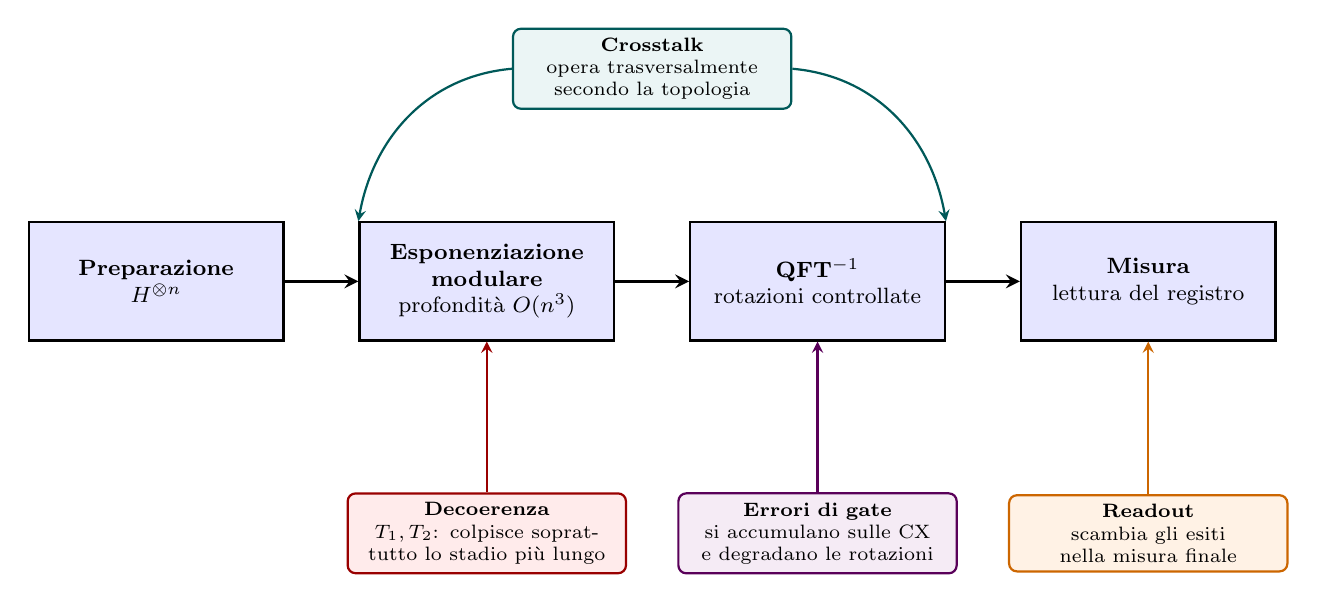
\begin{tikzpicture}[>=stealth,
  stage/.style={rectangle,draw=black,thick,fill=blue!10,minimum height=15mm,text width=30mm,align=center,font=\footnotesize},
  err/.style={rectangle,draw,thick,text width=33mm,align=center,font=\scriptsize,rounded corners=1mm},
  flow/.style={->,very thick}]
\node[stage] (S1) at (0,0) {\textbf{Preparazione}\\$H^{\otimes n}$};
\node[stage] (S2) at (4.2,0) {\textbf{Esponenziazione modulare}\\profondità $O(n^3)$};
\node[stage] (S3) at (8.4,0) {\textbf{QFT$^{-1}$}\\rotazioni controllate};
\node[stage] (S4) at (12.6,0) {\textbf{Misura}\\lettura del registro};
\draw[flow] (S1)--(S2); \draw[flow] (S2)--(S3); \draw[flow] (S3)--(S4);
\node[err,draw=red!60!black,fill=red!8] (E1) at (4.2,-3.2)
  {\textbf{Decoerenza}\\$T_1,T_2$: colpisce soprattutto lo stadio più lungo};
\node[err,draw=violet!70!black,fill=violet!8] (E2) at (8.4,-3.2)
  {\textbf{Errori di gate}\\si accumulano sulle CX e degradano le rotazioni};
\node[err,draw=orange!80!black,fill=orange!10] (E3) at (12.6,-3.2)
  {\textbf{Readout}\\scambia gli esiti nella misura finale};
\node[err,draw=teal!70!black,fill=teal!8] (E4) at (6.3,2.7)
  {\textbf{Crosstalk}\\opera trasversalmente secondo la topologia};
\draw[->,thick,red!60!black] (E1)--(S2);
\draw[->,thick,violet!70!black] (E2)--(S3);
\draw[->,thick,orange!80!black] (E3)--(S4);
\draw[->,thick,teal!70!black] (E4.west) to[out=185,in=80] (S2.north west);
\draw[->,thick,teal!70!black] (E4.east) to[out=-5,in=100] (S3.north east);
\end{tikzpicture}%
}
\caption[Dove colpisce il rumore nella pipeline di Shor]{Decoerenza, errori
di gate, readout e crosstalk colpiscono stadi differenti della pipeline.}
\label{fig:errori_shor}
\end{figure}

Nella \ac{QFT}, rotazioni sempre più piccole rendono critica la precisione di
fase; nella \ac{QPE}, il registro di controllo deve restare coerente lungo il
cammino causale dell'esponenziazione; nell'aritmetica modulare, l'elevato numero
di gate a due qubit accumula eventi. Sotto la sola ipotesi illustrativa di $L$
eventi indipendenti, il proxy di nessun evento è $(1-\epsilon)^L$: non è una
probabilità di successo algoritmico. Derivazione, esempio numerico e
Figura~\ref{fig:psuccess_vs_n} sono trasferiti nella
Sezione~\ref{app:shor_rumore_esteso}.

\section{Sfide Pratiche su Hardware NISQ}

La difficoltà operativa dipende insieme da qubit logici, routing e profondità.
Il circuito canonico $N=15$ usato qui, compilato nella base astratta
\texttt{rz/sx/x/cx}, contiene 224 \texttt{cx} e profondità 412; una mappatura
hardware aggiungerebbe routing dipendente dalla topologia. Le dimostrazioni di
$N=15$ e $N=21$ su dispositivi reali usano circuiti fortemente semplificati e
non generalizzabili~\cite{skosana2021}. Il seguito confronta quindi strategie
controllate: post-processing nella prima fase, poi \ac{QEC} e decodifica delle
sindromi, mantenendo distinti tassi logici e successo di Shor.

\end{onehalfspace}
